\paragraph{Passing variables}

Functions can also accept the values from variables as concrete values for their parameters. Let's study the following function:

\begin{minipage}[t]{0.5\textwidth}
\begin{nllisting}
void twice(text):
    print(text)
    print(text)
fruits = "pineapple blueberry"
twice(fruits)
\end{nllisting}
\end{minipage}
\begin{minipage}[t]{0.5\textwidth}
\begin{listing}
pineapple blueberry
pineapple blueberry
\end{listing}
\end{minipage}

We passed a single variable called \texttt{fruits} to the function. Its contents are named \texttt{text} inside the function definition. It is this text that is printed on the screen twice.

% Let er goed op dat een functie de waarde gebruikt die wordt meegegeven. Zo kan je buiten de functie een variabele hebben met dezelfde naam als een parameter van de functie. Bijvoorbeeld:
%
% \vspace*{-\baselineskip}\begin{verbatim}
% name = "david"
% void call(person):
%   print(person)
% call("sarah")
% \end{verbatim}\vspace*{-\baselineskip}
%
% Dit stukje code print \texttt{sarah}. Hoewel er buiten de functie de variabele \texttt{person} bestaat met de waarde \texttt{"david"}, wordt de functie aangeroepen met de string \texttt{"sarah"}. De waarde \texttt{"sarah"} wordt toegewezen aan de variabele \texttt{person}, en zo wordt uiteindelijk \texttt{sarah} geprint.

Like before, the order of the parameters will be consistent between the definition and any function calls that are performed. This is especially important because sometimes, parameters may have the same name as variables found elsewhere in the code. Consider this fragment:

\begin{nnflisting}
x = 10
y = 40
void minus(x, y):
    print(x - y)
minus(y, x)
\end{nnflisting}

Because the values of \texttt{y} and \texttt{x} are passed to the function in that order, inside the function we will have the concrete parameters \texttt{x = 40} and \texttt{y = 10}. Hence, the result that is printed will be 30.

\paragraph{Tracing}

Because of the potential confusion between variable and parameter names, we add an explicit step to our function tracing technique: substituting values in the function call. We cross out the variable name and write its value next to it. We can do this before considering the function's definition at all. Now that we have substituted the concrete values, it's easy to copy them into the concrete function call like in earlier sections.

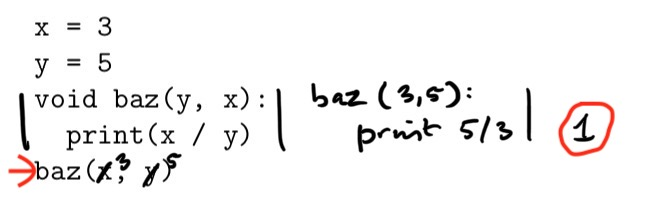
\includegraphics[width=.8\textwidth]{3-trace-varsparams.jpeg}
